\documentclass[conference]{IEEEtran}
% BranchLab manuscript. Compile with pdfLaTeX (Overleaf default).
\usepackage{cite}
\usepackage{amsmath,amssymb}
\usepackage{graphicx}
\usepackage{booktabs}
\usepackage{algorithm}
\usepackage{algpseudocode}
\usepackage{xcolor}
\usepackage{url}
\usepackage[hidelinks]{hyperref}

% Yellow placeholders to fill in before submission.
\newcommand{\fillin}[1]{\colorbox{yellow}{#1}}

\begin{document}

\title{BranchLab: Lightweight AST-Guided Boundary Test Generation for C, Java and Python}

\author{
\IEEEauthorblockN{Sneha Geevargis}
\IEEEauthorblockA{\textit{School of Computer Science and Engineering} \\
\textit{Vellore Institute of Technology}\\
Vellore, India \\
sneha.geevargis2024@vitstudent.ac.in}
\and
\IEEEauthorblockN{Sathya K}
\IEEEauthorblockA{\textit{School of Computer Science and Engineering} \\
\textit{Vellore Institute of Technology}\\
Vellore, India \\
\fillin{Faculty e-mail address}}
}

\maketitle

\begin{abstract}
Branch conditions are where off-by-one and wrong-operator faults hide, yet random inputs rarely land on a
condition's boundary, and generators based on symbolic execution, evolutionary search or large language models
need constraint solvers, long searches or external models. We present BranchLab, a lightweight test generator
that works entirely from the compiler front end. It parses a program into an abstract syntax tree (AST),
extracts variable--constant comparisons from \texttt{if}, \texttt{while} and \texttt{switch} statements, derives
boundary values for each, and combines them under a fixed test budget. Two techniques make the approach
practical across languages: a \emph{read map}, built from the AST, that delivers each generated value to the
input read it belongs to along that test's own path; and source-level \emph{probes} that measure branch and
statement coverage of compiled C and Java programs without an external coverage tool. We evaluate BranchLab on
15 programs in C, Java and Python against random testing with the same number of tests. AST-targeted suites
reached 90.0\% average branch coverage versus 57.6\%, 93.4\% statement coverage versus 70.1\%, and
detected 91.0\% of injected boundary mutants versus 14.1\%, with about 4~ms of generation time per
program. The benchmark also shows where the approach stops: conditions over sums, remainders or computed
values, and behaviour that needs a sequence of actions. BranchLab is open source and runs as a web application.
\end{abstract}

\begin{IEEEkeywords}
test case generation, abstract syntax tree, boundary value analysis, branch coverage, mutation testing,
program instrumentation
\end{IEEEkeywords}

\section{Introduction}
Software faults cluster at decision points. A threshold written as \texttt{>=} instead of \texttt{>}, or a
constant that is off by one, changes a program's behaviour only for inputs at the edge of a condition.
Boundary value analysis~\cite{myers2011art} has long recommended testing exactly those edges, and coverage
criteria such as branch coverage~\cite{zhu1997coverage} ask that every condition be observed both true and
false. In practice, test inputs are either written by hand, which is slow and gives no account of what was
missed, or drawn at random, which almost never lands on a specific boundary: for a guard such as
\texttt{age >= 18}, a uniform integer in $[-1000, 1000]$ equals 17, 18 or 19 with probability below 0.2\%.

Automated test generation research has answered this with powerful but heavy machinery. Concolic and symbolic
execution~\cite{godefroid2005dart,sen2005cute,cadar2006exe,cadar2008klee} solve path constraints with SMT
solvers and suffer path explosion; search-based
tools~\cite{korel1990automated,mcminn2004search,fraser2011whole,panichella2018dynamosa,lukasczyk2022pynguin}
evolve test suites over many fitness evaluations; and recent tools built on large language
models~\cite{lemieux2023codamosa,schafer2024testpilot,chen2024chatunitest} depend on large external models whose
tests must be checked and repaired. These techniques are valuable for complex software, but they are costly to
run, hard to explain, and usually tied to one language.

This paper takes the opposite, deliberately lightweight route. The compiler front end already exposes every
condition in a program as a node of its abstract syntax tree~\cite{aho2006compilers}. If a condition compares a
variable with a constant, the values that matter are known without solving anything: the constant and its
neighbours. BranchLab reads those conditions directly from the AST, generates boundary values, and runs and
measures the resulting tests for C, Java and Python. The contributions are:
\begin{itemize}
\item \emph{An AST-guided boundary test generator} that works through one pipeline for three languages, with
per-language adapters for parsing, analysis and execution, and links every test to the condition and line it
targets.
\item \emph{Path-aware input delivery:} a read map, derived from the AST, that answers each input read
(\texttt{scanf}, \texttt{Scanner}, \texttt{input()}) with the right generated value along the path that test
actually takes, including \texttt{switch} fall-through and helper functions.
\item \emph{Probe-based coverage for compiled languages:} a source-to-source transformation that measures branch
and statement coverage of C and Java programs with no external coverage tool, and survives \texttt{exit()},
crashes and timeouts.
\item \emph{An empirical comparison} with random testing on 15 programs, using branch coverage, statement
coverage, mutation score and generation time, including programs chosen to expose the approach's limits.
\end{itemize}
Section~\ref{sec:related} reviews related work, Section~\ref{sec:approach} presents the approach,
Section~\ref{sec:impl} the implementation, Section~\ref{sec:eval} the evaluation, Section~\ref{sec:threats}
threats to validity, and Section~\ref{sec:future} limitations and future work.

\section{Background and Related Work}\label{sec:related}
\subsection{Boundary Values, Coverage and Mutation Analysis}
Boundary value analysis selects inputs at and next to the edges of input domains~\cite{myers2011art}.
Structural coverage criteria measure how much of a program a test suite exercises: statement coverage counts
executed statements, while branch coverage counts the true and false outcomes of each decision and is strictly
stronger~\cite{zhu1997coverage}. Mutation analysis estimates fault-detection ability by seeding small syntactic
faults (mutants) and checking whether the suite distinguishes them from the
original~\cite{demillo1978hints,jia2011mutation}; mutants have been shown to be a valid substitute for real
faults in testing experiments~\cite{andrews2005mutation}.

\subsection{Automated Test Generation}
Random and feedback-directed random testing~\cite{pacheco2007randoop,arcuri2011art} is cheap and fully automatic
but has no structural targeting. DART~\cite{godefroid2005dart} and CUTE~\cite{sen2005cute} combine concrete and
symbolic execution; EXE~\cite{cadar2006exe} and KLEE~\cite{cadar2008klee} apply symbolic execution to systems
code in C. Search-based software testing~\cite{korel1990automated,mcminn2004search} treats input generation as
optimisation: EvoSuite~\cite{fraser2011whole} evolves whole test suites for Java,
DynaMOSA~\cite{panichella2018dynamosa} targets many coverage goals at once, and
Pynguin~\cite{lukasczyk2022pynguin} brings the approach to Python. Lakhotia et al.\ compared concolic and
search-based generation for C~\cite{lakhotia2010cute}. LLM-based tools such as
CodaMOSA~\cite{lemieux2023codamosa}, TestPilot~\cite{schafer2024testpilot} and
ChatUniTest~\cite{chen2024chatunitest} use language models to escape coverage plateaus or write tests directly.

\subsection{Positioning}
Table~\ref{tab:families} contrasts these families with BranchLab. Its targeted values come only from the AST:
there is no solver, no search loop and no model, generation takes milliseconds, and each test can be explained
by pointing at one condition. The price is a narrower class of conditions (Section~\ref{sec:future}); the gain
is an approach simple enough to apply uniformly to three languages and to teach.

\begin{table}[t]
\caption{Families of Automated Test Generation}\label{tab:families}
\centering\footnotesize
\begin{tabular}{@{}lll@{}}
\toprule
Approach & Relies on & Main cost \\
\midrule
Random~\cite{pacheco2007randoop,arcuri2011art} & random inputs & misses boundaries \\
Concolic / symbolic~\cite{godefroid2005dart,cadar2008klee} & constraint solver & path explosion \\
Search-based~\cite{fraser2011whole,panichella2018dynamosa} & fitness-guided search & many executions \\
LLM-based~\cite{lemieux2023codamosa,schafer2024testpilot} & language model & checking, repair \\
\textbf{BranchLab} & \textbf{AST conditions only} & narrower conditions \\
\bottomrule
\end{tabular}
\end{table}

\begin{figure*}[t]
\centering
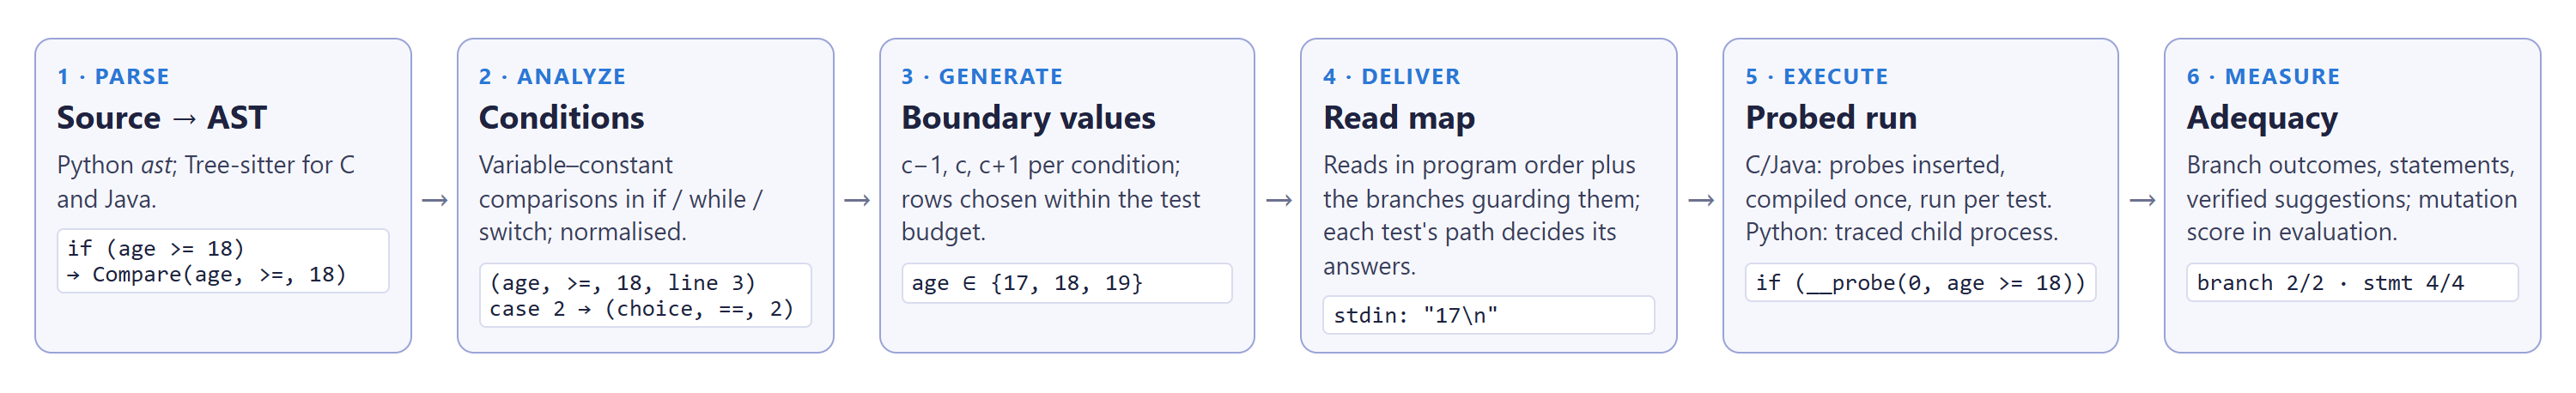
\includegraphics[width=\textwidth]{figures/approach.png}
\caption{BranchLab's pipeline, shown on the guard \texttt{age >= 18}. Each stage is implemented once and
specialised by a small per-language adapter.}
\label{fig:approach}
\end{figure*}

\section{Approach}\label{sec:approach}
Fig.~\ref{fig:approach} summarises the pipeline. A language adapter supplies four operations---parse, analyze,
plan inputs and execute---and everything else (test planning, coverage summaries, suggestions) is shared.

\subsection{Condition Extraction}
Python programs are parsed with the standard \texttt{ast} module; C and Java with Tree-sitter
grammars~\cite{treesitter}. The analyzer walks the tree and records every comparison between a variable and a
numeric constant in \texttt{if}, \texttt{else if}, \texttt{while} and \texttt{do-while} conditions, as a tuple
(variable, operator, constant, line). It normalises the forms programmers actually write: reversed operands
(\texttt{18 <= age} becomes \texttt{age >= 18}), negation, conjunctions and disjunctions (each atomic comparison
is kept), and signed, hexadecimal and suffixed literals such as \texttt{-5}, \texttt{0x1F}, \texttt{10L} or
\texttt{2.5f}. Each case of a \texttt{switch} statement (or Python \texttt{match} statement) on a variable
becomes an equality condition, so \texttt{case 2} yields \texttt{choice == 2}. Constructs the analyzer cannot
target, such as a \texttt{for} loop or a condition comparing two variables, are reported as untracked rather
than guessed.

\subsection{Boundary Values and Budgeted Combination}
For a condition $x \mathbin{op} c$ with integer $c$ the candidates are $c-1$, $c$ and $c+1$; for a
floating-point constant they are the nearest representable values on either side of $c$. Candidates are ordered
so that the second always satisfies the condition (18 for \texttt{age >= 18}, 6 for \texttt{x > 5}). A
variable constrained by several conditions receives the union of their candidates.

With several variables, the full product of candidates can exceed the test budget $k$. Rows are then chosen in
priority order (Algorithm~\ref{alg:rows}): first diagonal rows, which place every variable at its $i$-th
candidate; then rows that change one variable at a time, starting from the diagonal whose values all satisfy
their conditions, so that nested branches are reached and each variation flips exactly one of them; and finally
evenly spaced rows of the full product.

\begin{algorithm}[t]
\caption{Budgeted row selection}\label{alg:rows}
\begin{algorithmic}[1]
\Require candidate lists $V_1,\dots,V_n$; budget $k$
\State $S \gets [\,]$ \Comment{\textsc{Add} skips duplicates, stops at $|S|=k$}
\For{$i \gets 0$ \textbf{to} $\max_j |V_j| - 1$}
  \State \Call{Add}{$(V_1[i \bmod |V_1|], \dots, V_n[i \bmod |V_n|])$}
\EndFor
\For{each diagonal row $b$, satisfying diagonal first}
  \For{each variable $j$ and each $v \in V_j$, $v \neq b_j$}
    \State \Call{Add}{$b$ with position $j$ set to $v$}
  \EndFor
\EndFor
\For{$s \gets 0$ \textbf{to} $k-1$}
  \State \Call{Add}{product row $\lfloor s \cdot \prod_j |V_j| / k \rfloor$}
\EndFor
\State \Call{Add}{remaining product rows, in order}
\State \Return $S$
\end{algorithmic}
\end{algorithm}

Two further categories are optional: invalid-input tests (non-numeric text, empty input) and fuzz tests
(extreme magnitudes). They are reserved slots within the same budget and are labelled separately in the
results, so they never inflate targeted coverage.

\subsection{Path-Aware Input Delivery}
Generated values are keyed by variable name, but programs consume input by position: the first
\texttt{scanf}, the next \texttt{Scanner} call. Feeding values in a fixed order breaks as soon as different
paths read different variables---a menu option that reads an account number and an amount must not receive the
name that another option reads. BranchLab therefore builds a read map from the AST: the sequence of input reads
in program order, each tagged with the variable it assigns and its kind (integer, float, token, line),
interleaved with the branches and \texttt{switch} cases that guard them. Calls to helper functions are inlined.
For each test the map is resolved against that test's own values, following the branches they select
(including \texttt{switch} fall-through), to produce exactly the answers that path will read. Reads of
variables no condition mentions receive typed placeholders (\texttt{1}, \texttt{1.0}, \texttt{test}), so later
values are not shifted into the wrong variable. The answers go to standard input, command-line arguments or,
for Python, to the \texttt{input()} function inside the child process.

\subsection{Probe-Based Coverage for C and Java}
Python coverage is recorded by a tracer in the child process that runs each test. Compiled programs cannot be
traced that way, so BranchLab instruments the source before compiling it. Every tracked condition is wrapped in
a probe that records its identifier and outcome and returns the outcome unchanged, and every statement is
preceded by a line probe:
\begin{verbatim}
if (age >= 18) adult = 1;
   =>
if (__probe(0, (age >= 18))) {
    __line(4); adult = 1; }
\end{verbatim}
Unbraced bodies are wrapped in braces so the line probe stays inside the branch. Hits are appended to a file
named by an environment variable the moment they first occur, so outcomes survive \texttt{exit()}, crashes and
timeouts. In C a \texttt{\#line 1} directive after the probe prelude keeps compiler diagnostics on the user's
line numbers. The program is compiled once per run and executed once per test; if the instrumented build fails,
the plain build is used and coverage is reported as unmeasured rather than as zero.

\subsection{Verified Suggestions}
For every branch outcome left uncovered, BranchLab proposes an input that should reach it, runs that input once,
and labels it \emph{verified} only if the outcome really occurred; otherwise it is labelled \emph{not reached},
for example when the outcome sits behind another condition. Coverage figures are therefore never accompanied by
suggestions that would not work.

\section{Implementation}\label{sec:impl}
BranchLab is written in Python (about 4,391 lines for analysis, generation, execution, coverage and
evaluation) with a React web interface (about 2,255 lines) served by a FastAPI back end. Tree-sitter 0.25.2
parses C and Java; version 0.26.0 was found to return corrupted nodes and crash on large \texttt{switch}
statements, a regression the test suite guards against. Each Python test runs in a fresh process with a 3~s
limit; compiled tests have a 10~s limit. The tool is checked by 252 automated tests, which compare program
outputs with reference implementations and recompute expected branch outcomes independently instead of trusting
the reported coverage. The interface (Fig.~\ref{fig:ui}) shows each generated test with its category, inputs,
output and status, and a coverage view listing missed outcomes, untracked constructs and verified suggestions.
A Docker image bundles GCC and a JDK; a public instance runs at
\url{https://branchlab-ggon.onrender.com}.

\begin{figure}[t]
\centering
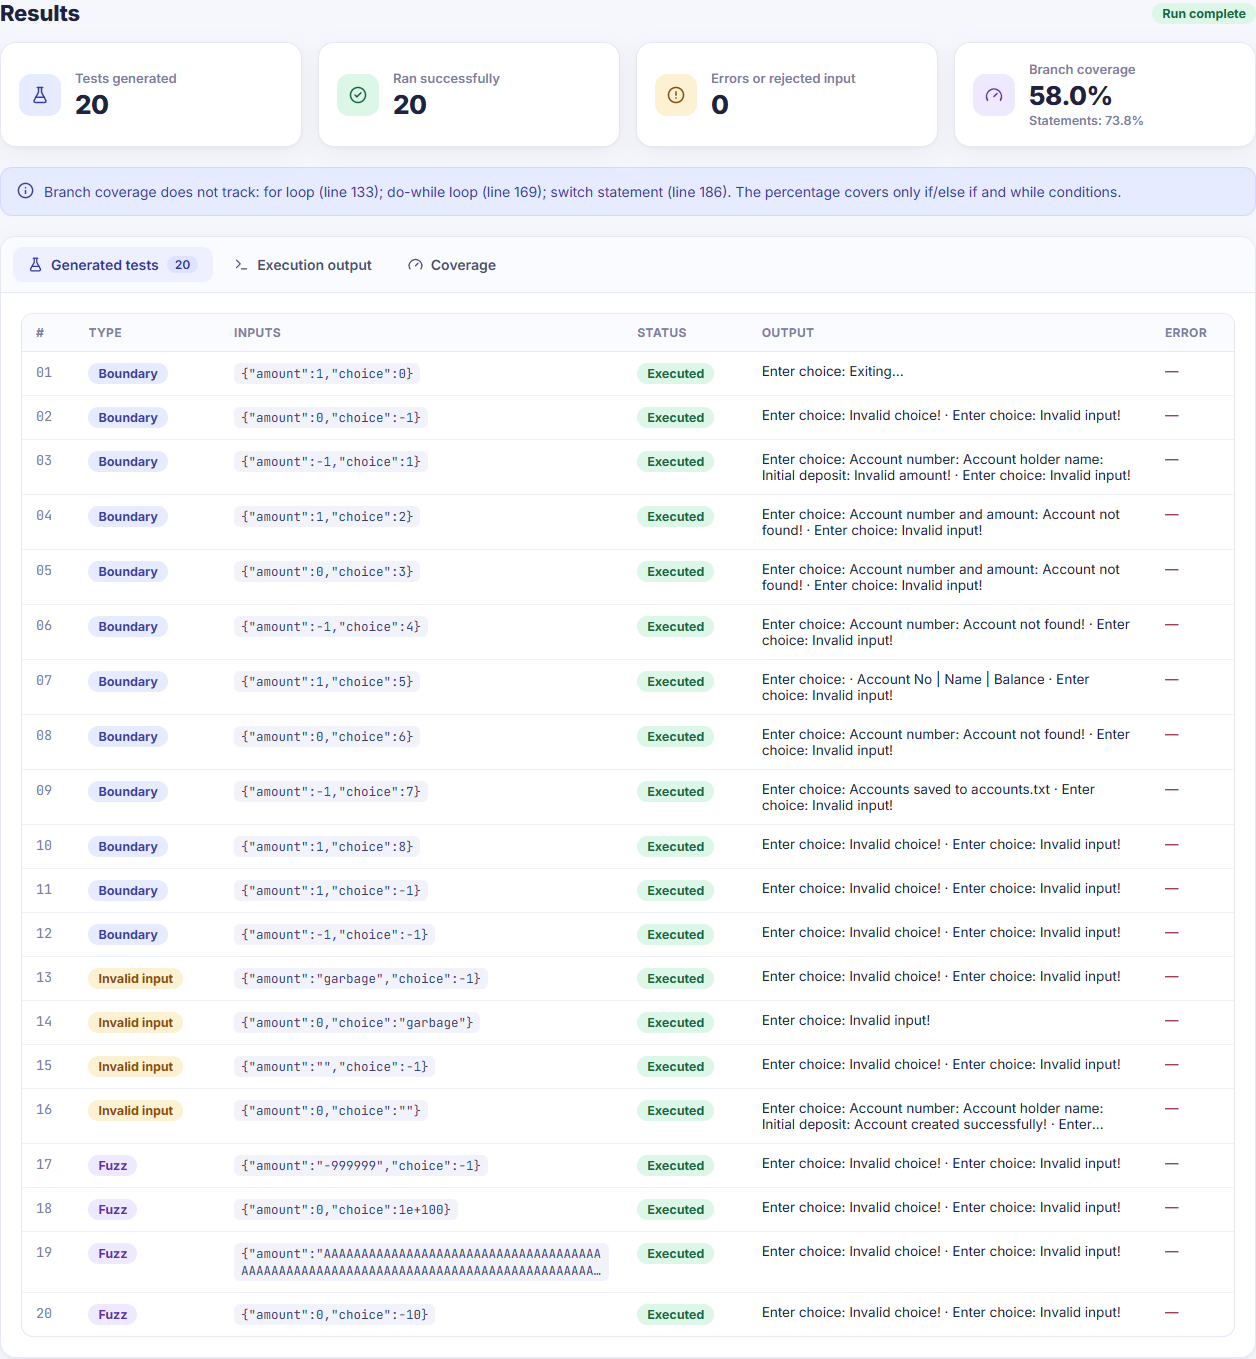
\includegraphics[width=\columnwidth]{figures/ui-bank-tests.png}
\caption{BranchLab running the C bank-management program: each generated test with its category, inputs,
status and output.}
\label{fig:ui}
\end{figure}

\section{Evaluation}\label{sec:eval}
The evaluation answers four research questions:
\begin{itemize}
\item \textbf{RQ1 (coverage):} Do AST-targeted suites reach higher branch and statement coverage than random
suites of the same size?
\item \textbf{RQ2 (fault detection):} Do they detect more boundary faults, measured by mutation score?
\item \textbf{RQ3 (cost):} How long does generation take, and how many tests are produced?
\item \textbf{RQ4 (limits):} On which programs does the approach fail, and why?
\end{itemize}

\subsection{Subject Programs}
Table~\ref{tab:subjects} lists the 15 subjects. Nine are BranchLab's example programs, including a
227-line menu-driven bank system in C; six are common programming-lab exercises added for this study,
three of them chosen because they contain conditions the approach cannot target: sums of variables (triangle),
remainders (leap year) and a value computed from the input (electricity bill).

\begin{table}[t]
\caption{Subject Programs}\label{tab:subjects}
\centering\footnotesize
\begin{tabular}{@{}llrrr@{}}
\toprule
Program & Lang. & LOC & Cond. & Tests \\
\midrule
\texttt{grade.py} & Python & 12 & 5 & 15 \\
\texttt{thermostat.py} & Python & 8 & 2 & 6 \\
\texttt{countdown.py} & Python & 6 & 1 & 3 \\
\texttt{nested\_login.py} & Python & 12 & 2 & 9 \\
\texttt{Grade.java} & Java & 17 & 5 & 15 \\
\texttt{Thermostat.java} & Java & 15 & 2 & 6 \\
\texttt{grade.c} & C & 18 & 5 & 15 \\
\texttt{countdown.c} & C & 12 & 1 & 3 \\
\texttt{bank.c} & C & 227 & 12 & 20 \\
\texttt{shipping.py} & Python & 17 & 6 & 20 \\
\texttt{leap\_year.py} & Python & 12 & 1 & 3 \\
\texttt{TaxSlab.java} & Java & 32 & 8 & 20 \\
\texttt{Calculator.java} & Java & 33 & 5 & 18 \\
\texttt{electricity\_bill.c} & C & 27 & 5 & 20 \\
\texttt{triangle.c} & C & 21 & 3 & 20 \\
\bottomrule
\end{tabular}
\end{table}

\subsection{Setup}
The targeted suite uses a budget of 20 tests and contains targeted tests only. The baseline draws uniform
integers in $[-1000, 1000]$ for the same input variables and produces exactly as many tests, so the comparison
isolates which values are chosen rather than how many; it is repeated with three fixed seeds and averaged. Both
suites are measured by the same instrumentation. Mutants apply three boundary operators at every comparison: the
relational operator shifted by one (\texttt{>} to \texttt{>=}, \texttt{<} to \texttt{<=}, \texttt{==} to
\texttt{!=}) and the constant plus or minus one. A mutant is killed when, for some test, the triple (executed,
output, first error line) differs from the original program's. In total 153 mutants were
generated, all of which compiled. Generation time covers AST analysis and input generation and excludes execution.
Experiments ran on a Windows 11 laptop with Python 3.13.13, GCC 16.1 and OpenJDK 25.

\begin{table*}[t]
\caption{AST-Targeted (AST) vs Random (Rnd) Suites of Equal Size}\label{tab:results}
\centering\footnotesize
\begin{tabular}{@{}lrrrrrrrrr@{}}
\toprule
 & & \multicolumn{2}{c}{Branch coverage} & \multicolumn{2}{c}{Statement coverage} & \multicolumn{2}{c}{Mutation score} & & \\
\cmidrule(lr){3-4}\cmidrule(lr){5-6}\cmidrule(lr){7-8}
Program & Tests & AST & Rnd & AST & Rnd & AST & Rnd & Mutants & Gen.\ ms \\
\midrule
\texttt{grade.py} & 15 & 100.0\% & 29.2\% & 100.0\% & 43.3\% & 100.0\% & 0.0\% & 15 & 0.6 \\
\texttt{thermostat.py} & 6 & 100.0\% & 75.0\% & 100.0\% & 83.3\% & 100.0\% & 0.0\% & 6 & 0.4 \\
\texttt{countdown.py} & 3 & 100.0\% & 100.0\% & 100.0\% & 100.0\% & 100.0\% & 100.0\% & 3 & 0.8 \\
\texttt{nested\_login.py} & 9 & 100.0\% & 83.3\% & 100.0\% & 90.5\% & 100.0\% & 0.0\% & 6 & 0.5 \\
\texttt{Grade.java} & 15 & 100.0\% & 29.2\% & 100.0\% & 43.3\% & 100.0\% & 0.0\% & 15 & 10.1 \\
\texttt{Thermostat.java} & 6 & 100.0\% & 75.0\% & 100.0\% & 85.7\% & 100.0\% & 0.0\% & 6 & 2.0 \\
\texttt{grade.c} & 15 & 100.0\% & 29.2\% & 100.0\% & 48.5\% & 100.0\% & 0.0\% & 15 & 7.4 \\
\texttt{countdown.c} & 3 & 100.0\% & 100.0\% & 100.0\% & 100.0\% & 100.0\% & 100.0\% & 3 & 0.7 \\
\texttt{bank.c} & 20 & 48.0\% & 6.0\% & 69.7\% & 15.2\% & 50.0\% & 11.1\% & 12 & 11.9 \\
\texttt{shipping.py} & 20 & 100.0\% & 70.0\% & 100.0\% & 81.0\% & 100.0\% & 0.0\% & 18 & 6.6 \\
\texttt{leap\_year.py} & 3 & 62.5\% & 58.3\% & 70.0\% & 66.7\% & 100.0\% & 0.0\% & 3 & 1.0 \\
\texttt{TaxSlab.java} & 20 & 100.0\% & 72.2\% & 100.0\% & 84.8\% & 75.0\% & 0.0\% & 24 & 11.6 \\
\texttt{Calculator.java} & 18 & 100.0\% & 0.0\% & 100.0\% & 44.4\% & 100.0\% & 0.0\% & 3 & 5.9 \\
\texttt{electricity\_bill.c} & 20 & 90.0\% & 86.7\% & 89.5\% & 93.0\% & 40.0\% & 0.0\% & 15 & 1.6 \\
\texttt{triangle.c} & 20 & 50.0\% & 50.0\% & 71.4\% & 71.4\% & 100.0\% & 0.0\% & 9 & 1.1 \\
\midrule
\textbf{Mean} & 12.9 & \textbf{90.0\%} & 57.6\% & \textbf{93.4\%} & 70.1\% & \textbf{91.0\%} & 14.1\% & 10.2 & 4.2 \\
\bottomrule
\end{tabular}
\end{table*}

\begin{figure*}[t]
\centering
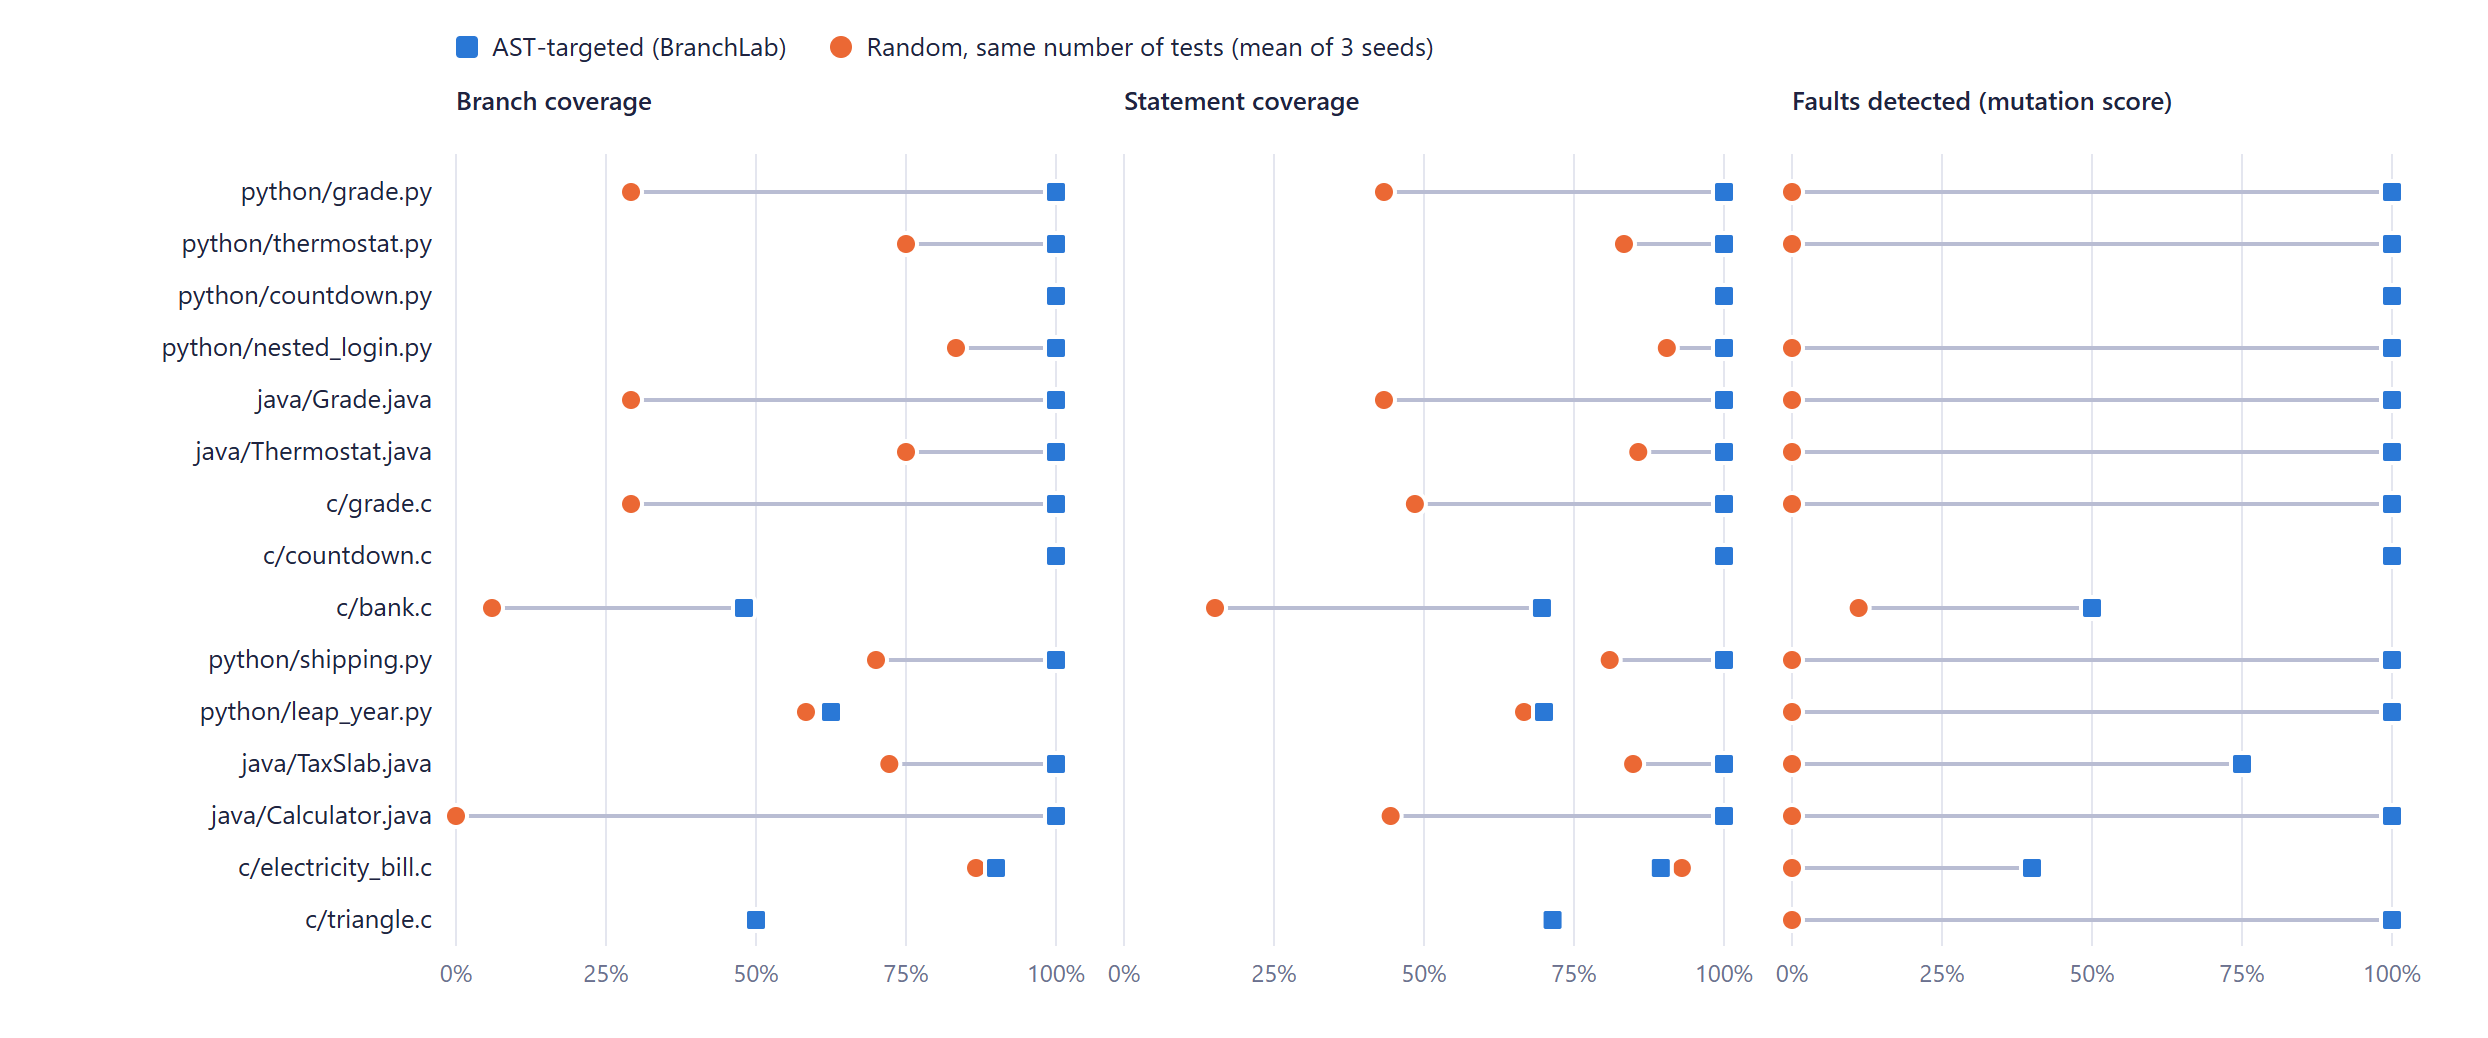
\includegraphics[width=\textwidth]{figures/comparison.png}
\caption{Per-program comparison. Squares: AST-targeted suite; circles: random suites of the same size (mean of
three seeds). A square to the right of its circle means the targeted suite did better on that program; where
only a square is visible, both suites scored the same.}
\label{fig:comparison}
\end{figure*}

\subsection{Results}
\textit{RQ1 (coverage).} Averaged over the 15 programs, the targeted suites reached 90.0\% branch coverage
against 57.6\% for random suites, and 93.4\% statement coverage against 70.1\%
(Table~\ref{tab:results}, Fig.~\ref{fig:comparison}). Branch coverage was higher on 12 programs and equal
on 3, and never lower (exact Wilcoxon signed-rank test, $p<0.001$). For statement coverage the targeted
suite won on 11 programs, tied on 3 and lost on 1 ($p=0.001$). Random suites do well only
where any value in a wide range satisfies or violates a condition, as in the countdown loops.

\textit{RQ2 (fault detection).} The targeted suites killed 91.0\% of mutants on average against 14.1\%; they
were better on 13 programs and equal on 2 ($p<0.001$). The gap is far larger than the coverage gap,
because covering a branch is not enough to expose a boundary fault: a random suite can execute both sides of
\texttt{age >= 18} without ever testing 17, 18 or 19, so a mutant \texttt{age > 18} survives. Fault detection is
where boundary values matter most.

\textit{RQ3 (cost).} Analysis and generation took 4.2~ms per program on average and at most 11.9~ms.
Suites contained 3 to 20 tests (mean 12.9); small programs need far fewer than the
budget because the full candidate product is small. Random generation is cheaper still, but at equal size its
tests are far less effective. Execution, not generation, dominates the end-to-end time, chiefly JVM start-up
for Java.

\textit{RQ4 (limits).} The benchmark shows four ways the approach falls short. (i) \emph{Relations between
variables:} in \texttt{triangle.c} the checks \texttt{a + b <= c} are not variable--constant comparisons; both
suites reached 50.0\% branch coverage. (ii) \emph{Arithmetic in conditions:} in \texttt{leap\_year.py},
\texttt{year \% 400 == 0} yields no candidates, leaving the suite at 62.5\%. (iii) \emph{Computed values:} in
\texttt{electricity\_bill.c} the surcharge depends on \texttt{bill > 1000}, where \texttt{bill} is computed from
\texttt{units}; BranchLab produces boundary values for \texttt{bill}, but no input sets it, and the random suite
reached more statements (93.0\% vs 89.5\%) because large random readings trigger the surcharge.
(iv) \emph{Stateful sequences:} in \texttt{bank.c} many branches need several actions in one run (create an
account, then deposit), which no single-shot suite generates; the targeted suite reached 48.0\% branch
coverage against 6.0\%. Menu programs also explain the largest gaps in Table~\ref{tab:results}: in
\texttt{Calculator.java} the \texttt{switch} cases themselves are not yet counted as branches, and the one
measured condition (\texttt{b == 0}) sits under \texttt{case 4}, which no random suite selected, leaving random
suites at 0.0\% branch coverage.

\section{Threats to Validity}\label{sec:threats}
\textit{Construct validity.} The mutation operators are boundary faults, the class of fault the approach
targets; scores for other fault classes (missing statements, wrong variables) would be lower and closer between
the two techniques. Some mutants may be equivalent, so a score below 100\% is not always a missed fault.

\textit{Internal validity.} The random range $[-1000, 1000]$ affects the baseline: a narrower range would hit
small constants more often. The range is wide enough to cross every constant in the subjects; the baseline also
receives exactly as many tests and is averaged over three seeds. The same instrumentation measures both suites.

\textit{External validity.} The 15 subjects are small, input-driven programs, all written for this project;
results may not carry over to large programs, programs driven by files or networks, or object-oriented code
under unit test. The benchmark deliberately includes programs where the approach fails to limit this bias.

\section{Limitations and Future Work}\label{sec:future}
Each test is a single run with one set of values, so behaviour that needs a sequence of actions is not
generated; sequence generation guided by the read map is the most valuable extension. Only variable--constant
comparisons produce targeted values; lightweight constraint handling for relations such as \texttt{x > y} and
for simple arithmetic (\texttt{x \% 4 == 0}) would cover the triangle and leap-year cases without a full solver.
Values computed from inputs could be handled by propagating boundaries back through straight-line assignments.
Branch coverage does not yet count \texttt{for} loops, \texttt{switch} cases and the conditional operator, which
the interface lists as untracked. Finally, process isolation contains hangs and crashes but is not a security
sandbox; container sandboxing would be needed for an open public service.

\section{Conclusion}
BranchLab shows that the compiler front end alone carries enough information to generate effective boundary
tests. Reading conditions from the AST, delivering values along each test's own path and measuring coverage with
source probes gives one lightweight pipeline for C, Java and Python. Against random suites of equal size it
raised average branch coverage from 57.6\% to 90.0\% and boundary-fault detection from 14.1\% to
91.0\%, in milliseconds and with every test traceable to its condition. Its failures are equally clear and
point to the next steps: relations between variables, arithmetic in conditions, and input sequences for
stateful programs. Source code, benchmark programs and evaluation scripts are available at
\url{https://github.com/SnehaGEE/ast-test-generator}.

\section*{Acknowledgment}
The authors thank the School of Computer Science and Engineering, Vellore Institute of Technology, for its
support of this work, carried out as part of the BCSE307P Compiler Design Lab course.

\bibliographystyle{IEEEtran}
\bibliography{refs}

\end{document}
